\section{Further Analysis}\label{sec:ControllerVerification}
Since the real implementation of the controller is not stable, a further analysis is done in this section.

The first step is to simulate both the continuous and discrete controller with the model of the system and analyse the behavior of the whole closed loop system.

This is done not only to see the behavior of the designed controller but also to verify that the discretized controller matches the original continuous one. 

With a constant reference of 0 rad and a disturbance in the form of a torque applied to the frame of \si{0,55 Nm}, the responses are the ones shown in \figref{discreteVsContinuousOutputController} and \figref{discreteVsContinuousSimulation}.
%
\begin{minipage}{0.45\linewidth}
	\begin{figure}[H]
      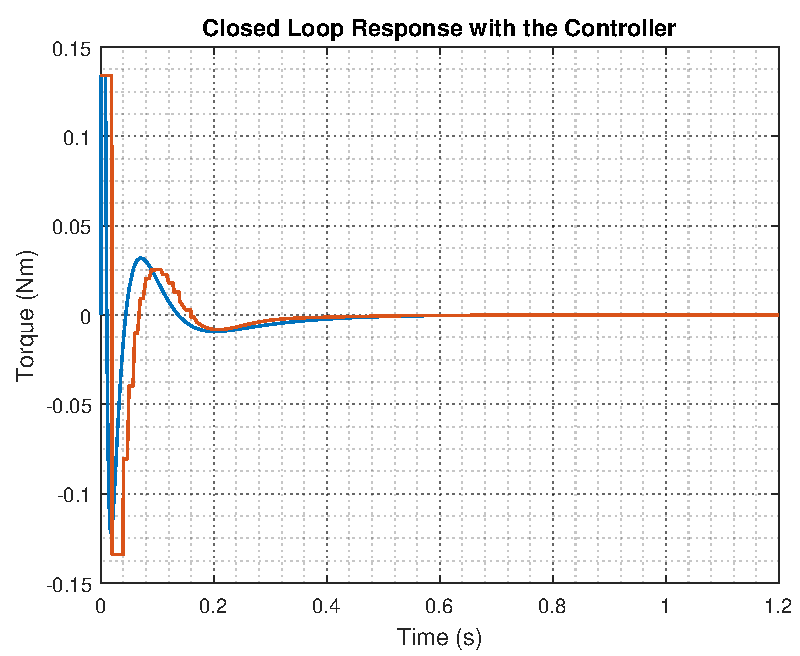
\includegraphics[scale=.53]{figures/torqueComp}
      \captionsetup{justification=centering}
      \captionof{figure}{Controller's output (torque) response in the control loop with the continuous (blue) and discrete (red) controllers}
      \label{discreteVsContinuousOutputController}
    \end{figure}\vspace{-5mm}
\end{minipage}
\hspace{0.03\linewidth}
\begin{minipage}{0.45\linewidth}
    \begin{figure}[H]\vspace{-4mm}
      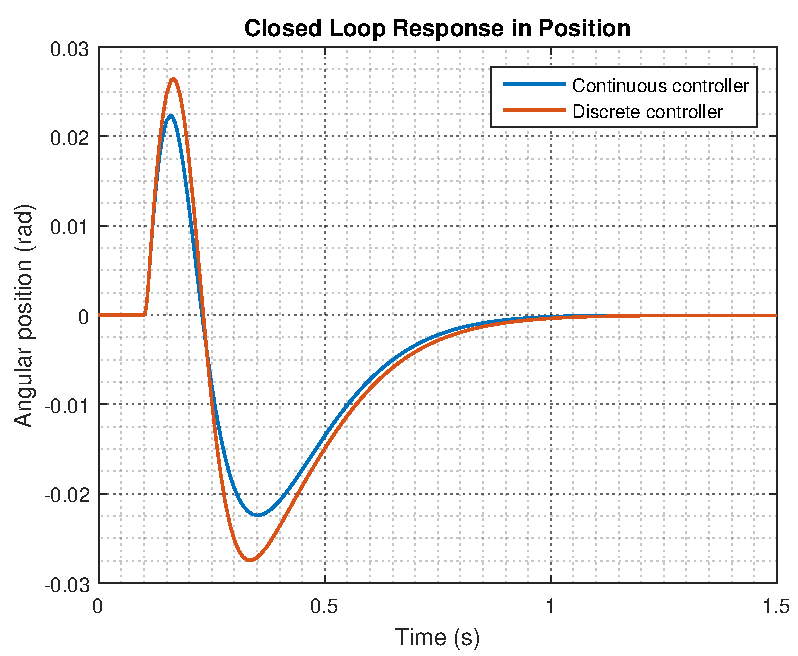
\includegraphics[scale=.53]{figures/positionComp}
      \captionsetup{justification=centering}
      \captionof{figure}{Closed loop response of the continuous (blue) and discrete (red) controllers}
      \label{discreteVsContinuousSimulation}
    \end{figure}\vspace{-5mm}
\end{minipage}

Both controllers seem to have a good behavior and both reach the desired final position in simulation when a disturbance is applied. On the contrary, the previously implemented controller is not even able to keep the Cubli in an equilibrium position with no disturbance. \\
%
\begin{figure}[H]\vspace{-4mm}
	\centering
	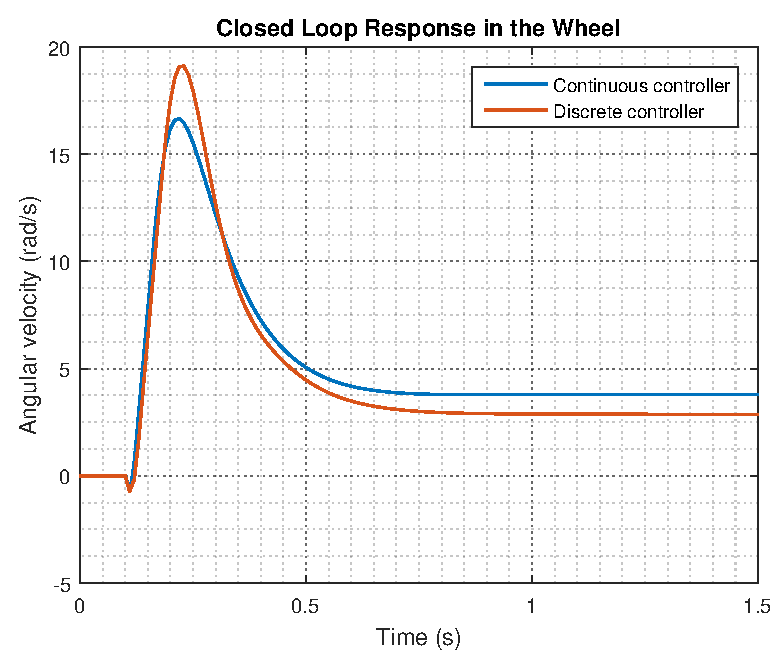
\includegraphics[scale=.53]{figures/wheelComp}
	\captionof{figure}{Angular velocity of the wheel from the simulation when a disturbance torque is applied. When angular position reaches steady state (\figref{discreteVsContinuousSimulation}) the value of the velocity is not \SI{0}{rad \cdot s^{-1}}.}
   \label{fig:discreteVsContinuousWheel}
\end{figure}\vspace{-5mm}

Anyhow, even in the simulation, the velocity of the wheel is different than 0 when the angle reaches a steady state as shown on \figref{fig:discreteVsContinuousWheel}.\\
It should not be any problem since a constant velocity does not produce any torque 
to the system. However there is friction in the wheel, which will make it to slow down, producing an acceleration on the system. This will make the Cubli to slightly move from equilibrium position and the controller will try to apply some torque to the system to balance it. The problem arises if the motor was already very closed to its maximum speed and it will not be able to accelerate more and produce the torque needed, making the frame fall over.

The conclusion is that a Single-Input Single-Output controller is not able to ensure zero velocity in equilibrium with only a feedback in the position of the frame. This means that another kind of controller, which also takes care of the velocity of the wheel, may result in a better behavior.

One way could be using a cascade controller to control both the velocity of the wheel and the position of the frame. In \figref{cascadeControl} it can be seen the block diagram for a cascade control, with the particularity of a feedback from the position of frame to the velocity of the wheel.

\begin{figure}[H]
	  \begin{tikzpicture}[ auto,
thick,                         %<--setting line style
node distance=2cm,             %<--setting default node distance
scale=1.0,                     %<--|these two scale the whole thing
every node/.style={scale=1.0}, %<  |(always change both)
>=triangle 45 ]                %<--sets the arrowtype
  ]
  
  %-- Blocks creation --%
  \draw
	node[shape=coordinate][](ref) at (0,0){\si{\theta_F}}			% start of reference
 
	node(sum1) at (2,0) [sum] {$\sum$}
 
	node(D2) at (4,0) [block] {$D2$}
	
	node(sum2) at (6,0) [sum] {$\sum$}
	
	node(D1) at (8,0) [block] {$D1$}
	
	node(G1) at (10,0) [block] {$G1$}
	
	node[shape=coordinate][](velFeed) at (11,0){omega\_f}
	
	node(G2) at (12,0) [block] {$G2$}
	
	node[shape=coordinate][](feed) at (13,0){feed}
	
	node[shape=coordinate][](angleFeed) at (14,0){theta\_f}
	
	node[shape=coordinate][](out) at (15,0){theta\_f}
	
	% - feedback nodes
	
	node[shape=coordinate][](feed1) at (9,-1.5){feed1}
	
	node[shape=coordinate][](feed2) at (9,-2){feed2}
	
	node[shape=coordinate][](feed3) at (12,-1){feed3}
	
  ;
  
  \draw[->](ref) -- node {\si{\theta_F}} (sum1);
  
  \draw[->](sum1) -- node {} (D2);
  
  \draw[->](D2) -- node {} (sum2);
  
  \draw[->](sum2) -- node {} (D1);
  
  \draw[->](D1) -- node {} (G1);
  
  \draw[->](G1) -- node {\si{\dot{\theta}_F}} (G2);
  
  \draw[->](G2) -- node {\si{\theta_F}} (out);
  
  % - drawing feedback lines
  
  \draw[-](velFeed) |- node {} (feed1);
  
  \draw[-](angleFeed) |- node {} (feed2);
  
  \draw[-](feed1) -| node {} (sum2);
   
  \draw[-](feed2) -| node {} (sum1);
  
  \draw[dashed](feed) |- node {} (feed3);
  
  \draw[dashed, ->](feed3) -| node {} (G1);
  
  % - adding + and - at the sum nodes
    \draw
  node at (sum1) [right = -6.6mm, below = .6mm] {$+$}
  node at (sum1) [right = -3mm, below = 3.9mm]  {$-$} 
  
  node at (sum2) [right = -6.6mm, below = .6mm] {$+$}
  node at (sum2) [right = -3mm, below = 3.9mm]  {$-$} 
  ;
 
  
  \end{tikzpicture}
	\centering
	\caption{Block diagram for a cascade control (the dotted line corresponds to a feedback in the Cubli system that is not present in the normal cascade control)}
	\label{cascadeControl}
\end{figure}

The problem of this solution in the case of the Cubli is that both variables to control are coupled together, which means that it is not possible to split the plant in a way that there is no feedback between them.\cite{LRusso}

Another way is to use a state space approach, which can handle this singularity, since now the system will have two outputs to control. This controller solution is further detailed in \chapref{chap:stateSpaceController}.
